\input{tables/ArXivqa}

\section{Experiments}

We conduct experiments to (i) validate the effectiveness of ArXivQA for boosting multimodal scientific reasoning for open-source LVLMs~(\S\ref{subsec:math_reasoning}) and (ii) benchmark LVLMs capability to comprehend scientific figures with ArXivCap~(\S\ref{subsec:exp_arxivcap}).


\subsection{Boosting LVLMs with ArXivQA}
\label{subsec:math_reasoning}

\subsubsection{Experimental Settings}
\label{subsubsec:exp_setting}
We adopt Qwen-VL-Chat-7B~\citep{Qwen-VL}
as the backbone due to its support for interleaved image-text input formats and high-resolution images.
We fine-tune it on our ArXivCap (Qwen-VL-Chat-7B$_\text{ArXivCap}$), ArXivQA (Qwen-VL-Chat-7B$_\text{ArXivQA}$) and combination of these two datasets (Qwen-VL-Chat-7B$_\text{ArXivCap + ArXivQA}$) for three epochs with a learning rate of 1e-5 following the original paper.
We combine the answer and the rationale in ArXivQA to form the target output during training. 
Models are evaluated on MathVista~\citep{mathvista}, a benchmark that requires fine-grained, deep visual understanding and compositional reasoning. MathVista contains 6,141 examples, consisting of five multimodal tasks Figure QA, Geometry Problem Solving, Math word problem, Text Book QA, and Visual QA. 
We select 478 multiple-choice questions in the \texttt{testmini} split to avoid the inconsistency of answer parsing. We compute the accuracy scores and adopt the provided prediction files for calculating the baseline performance.
% is adopted as the metric.

\subsubsection{Results}

As shown in Table~\ref{tab:mathvista_ret},
fine-tuning on our Multimodal ArXiv, especially on the ArXivQA dataset, consistently boosts the performance, helping the open-sourced Qwen-VL-Chat achieve a comparable overall MathVista reasoning performance.
Due to the wide coverage of the scientific figures, the performance gain mainly comes from significantly improved Geometry Problem Solving, Textbook QA, and Visual QA tasks. For example, after fine-tuning on the ArXivQA dataset, the accuracy is increased from 19.1\% to 34.0\% and from 46.7\% to 70.0\% on Geometry Problem Solving and Textbook QA tasks, respectively.
The improvement on Math Word Problem is marginal, where we think the domain-specific data augmentation can be further explored with a curated filtering dataset on our dataset~\citep{gao2023gllava}.
On the contrary,
the accuracy of Figure QA deteriorates slightly compared with the original backbone model, which we attribute to the fact that most of the plots in the Figure QA evaluation are sampled from synthesized datasets such as DVQA~\citep{kafle2018dvqa}, exhibiting great gaps between real-world paper figures.

\subsubsection{Analysis}
We investigate how different subject domains affect mathematical reasoning ability using pairs of questions and answers (QA). We focus on six domains with more than 5K samples each. From each domain, we randomly choose a subset of 5K samples to ensure fairness in comparison. We then fine-tune the Qwen-VL-Chat base model using QA pairs from each domain and observe how it affects the model's accuracy compared to its original state.
Figure~\ref{fig:domain_analysis} demonstrates the relative accuracy changes (i.e., $\frac{\text{Accuracy after Fine-tuning}}{\text{Original Accuracy}} - 1 $) after training the model on QA pairs from each domain. Our findings reveal several key points: (i) QA pairs from the Computer Science (CS) domain are highly effective for improving mathematical reasoning ability, achieving a notable 27.09\% relative improvement. We attribute this to the compositional nature of the CS area. (ii) The most beneficial domain varies depending on the specific task. For instance, QA pairs from astrophysics domains enhance geometry problem-solving, while those from Condensed Matter improve performance in math word problems. (iii) Most domains hurt the Figure QA task. This suggests that synthetic Figure QA might not be the best benchmark for assessing realistic reasoning ability.
These findings underscore the efficacy of generated QA pairs and offer valuable insights for future research, such as adjusting task-specific weights in the dataset accordingly.



\section{The CC-Layer}
\label{sec:implement}
\subsection{Constructing the CC-layer}
\label{sec:implement_construct}
Given a discrete feature map $\varbold{I}$ of shape $[N,C_{in},H,W]$, we are interested in a layer that produces $\varbold{I'}=CC\{\varbold{I}\}$ of shape $[N,C_{out},H',W']$ which is resized by a (non-integer) scale-factor $(s_h, s_w)$. Here $N$ is the batch-size, $C$ is the number of channels. $H,W$ are spatial dimensions. The desired spatial size $H',W'$ may be chosen at inference time.
Our CC-layer consists of 4 principled building blocks, marked by numbers in Fig.~\ref{fig:overview} (for simplicity, $I$ and $I'$ are drawn as 2D vectors in Fig.~\ref{fig:overview}, i.e.,  4D tensors with $N=1$ and $C=1$). These are described next:

\textbf{Block 1 -- Projected-grid:} 
The Projected grid \varbold{$\textbf{g}$} matches each output `pixel' $\textbf{n}$=$(i', j')$$\in$$I'$ to a sub-`pixel' location \varbold{$\textbf{g}_n$} in the continuous space of the \ben{input} $I$. This grid is captured by a tensor of shape $[2,H',W']$ where the the first dimension are the 2 projected sub-`pixel' coordinates (vertical and horizontal) of each output `pixel' $\textbf{n}$=$(i', j')$$\in$$I'$, and $H', W'$ are for all the output `pixels'.

%\michal{why don't we see the number of Fig.4 in the next paragraph?}

Let's start with a simple example. Fig.~\ref{fig:grid}.a depicts a standard 1D  downscaling by %an integer 
$2$. Note that even when the scale-factor $s$ is an integer (or an inverse integer: ${s=\ben{\nicefrac{1}{2}}}$ in this case), it is  \emph{wrong} to map an output `pixel' position $\textbf{n}$$\in$$I'$  to its input position in $I$ by simply multiplying (or dividing)  by the scale-factor $s$. It can be observed in Fig.~\ref{fig:grid}.a   that ${\varbold{\textbf{g}_n}\neq2\textbf{n}=\textbf{n}}/{s}$
%\ben{\nicefrac{\textbf{n}}{s}}}$.
To obtain the correct mapping, let's
define $d_{out}$  to be the distance of any output `pixel'  
%\textbf{n}$$\in$$I'$  
\michal{$\textbf{n}$}
from the leftmost boundary of $I'$.  $d_{out}$  is measured in units of output `pixels'. The matching coordinates \varbold{$\textbf{g}_n$}   in the \ben{input} $I$  is  defined to have a distance $d_{in}$ from the leftmost boundary of  $I$, and is measured in units of input `pixels'. The correct mapping rule across image scales~\cite{MATLAB:2010} is $d_{in}$=${d_{out}}/{s}$, 
since the total shape (from boundary-to-boundary) is resized, rather than discrete `pixel' centers. Since the first `pixel' \emph{center} (in any \ben{feature map/image}) is always half a `pixel' away from the leftmost boundary, hence:
%we can easily relate $d$ to $n$ and to $\varbold{\textbf{g}_n}$, by 
$d_{out}$=$n$+$\frac{1}{2}$  and  $d_{in}$=$\varbold{\textbf{g}_n}$+$\frac{1}{2}$.
%Plugging it in, we get the
This entails the
well known relation used in image resizing methods~\cite{MATLAB:2010}: 
%$ \varbold{\textbf{g}_n}$=$\frac{n}{s}$+$\frac{1}{2}$$\left(\frac{1}{s}-1\right)$
$ \varbold{\textbf{g}_n}$=$\frac{n}{s}$+$\frac{1}{2}$$(\frac{1}{s}$-$1).$

% \michal{the next paragraph is very tedious, can and SHOULD be shortened substantially.}
% However, we need to handle also non-integer output shapes. Such an example is illustrated in Fig.~\ref{fig:grid}.b. Since images or feature-maps  can only be represented  by integer-sized vectors/tensors, we will usually (but not always) determine the size of the output layer to be $out\_size =\lceil s \cdot in\_size \rceil$, However, the intrinsic (non-integer) output size $s \cdot in\_size$ must be kept, as this is the true size of the output, while the integer size contains an extra sub-`pixel' margin. Fig.~\ref{fig:grid}.b shows a projected grid for resizing a $4 \times 4$ input layer by 0.6 and 1.4,  respectively. The final output size ($3 \times 6$) is larger than the intrinsic size ($2.4 \times 5.6$), due to the ceiling $\lceil * \rceil$ operation. 
% % To prevent misalignments, we need to map each output `pixel' center to its correct input `pixel' center. For this we need to shift the output `pixels' by half of the margin $\textbf{n}=\textbf{n}' -(out\_size - in\_size \cdot s)/2$. Plugging this into the relation of $p$ to $p'$ we obtain:
% To prevent misalignments due to this added sub-`pixel' output margin, and guarantee that each output `pixel' center is mapped to its correct input location, we need to shift the output `pixels' by half of the added margin:  $\textbf{n}=\textbf{n}' -(out\_size - in\_size \cdot s)/2$. %Plugging this into the relation of $p$ to $p'$ we obtain:
% This yields the final accurate grid mapping:
However, we need to handle also non-integer output shapes. The intrinsic output size 
$s \cdot in\_size$ may not be an integer, yet images or feature-maps  can only be represented  by integer-sized vectors/tensors. We will usually (but not always) determine the size of the output $I'$ to be $out\_size =\lceil s \cdot in\_size \rceil$. Fig.~\ref{fig:grid}.b shows an example of a projected grid for resizing a $4 \times 4$ input \ben{feature map} by scales 0.6 and 1.4,  respectively. The final output size ($3 \times 6$) is larger than the intrinsic size ($2.4 \times 5.6$), due to the ceiling operation $\lceil$*$\rceil$.  Therefore, the final  grid mapping (which accurately covers all cases) is:
\begin{align}
    \varbold{g_n} = \frac{n}{s} + \frac{1}{2}\Big( in\_size - 1\Big) - \frac{1}{2s}\Big(out\_size-1\Big)    
    \label{eq:grid}
\end{align}
% Since every output `pixel', (i, j) is mapped to continuous 2D coordinates in the input feature-map, % Since the grid matches two location coordinates to each output `pixel', 
% it is a represented as a standard CNN tensor of order 4, with shape $[1,2,H',W']$, where 
% the batch size is 1. The second dimension is 2 for 2 spatial continuous coordinates in the input space and the last two are for the height and width of the output. 


% First we calculate a grid of sub-pixel coordinates, which matches output pixels locations in the input continuous space. Each output pixel is assigned to horizontal and vertical sub-pixel position in the input. This grid is a function purely of the scale-factors and the output shape. Thus, importantly, the grid can be determined at inference time dynamically.

% To accurately obtain the projected-grid, we need to acknowledge that discrete `pixels' have non-infinitesimal size, thus we distinguish between `pixel' ordinal numbers to continuous locations of their centers. Fig.~\ref{fig:grid}.a depicts a 1d standard downscaling by a factor of $\frac{1}{2}$. Note that it even when the downscalinfg/upscalingis by an integer scale-factor (2 in this case), it is wrong to map output `pixel' positions to input positions by directly multiplying by the scale-factor. We mark the discrete `pixel' coordinates by $p$ and the scale-factor by $s$. First we observe that $p' \neq sp$. In the figure it is clear that `pixel' 0 should not be mapped to output `pixel' 0, rather the boundary between `pixel' 0 to `pixel' 1. We define the distance from the left boundary as $d$ measured in units of full `pixel's. Since the first `pixel' center is half a `pixel' to the right with respect to the left boundary, $d=p+\frac{1}{2}$. To correctly resize, we need the total size of the input (4 in the example) to be mapped to the total size of the output, hence $d'=s \cdot d$. plugging in the relation between $p$ and $d$: $p'+\frac{1}{2} = s(p+\frac{1}{2})$ so that the mapping rule between input and output `pixels' is $p = \frac{p'}{s} + \frac{1}{2} \left( \frac{1}{s} - 1 \right)$.


% Next we need to handle non-integer output shapes. Since we can only represent images or feature-maps sizes as integers we will usually (but not always) determine the output size as $Ceil(s \cdot in\_size)$. However, the intrinsic size $s \cdot in\_size$ must be held. We point out that in some cases of resizing, it is crucial to specify both scale-factors and output shape. For example, in a sequence of resizing operations. Fig.~\ref{fig:grid}.b illustrates projected grid for resizing by 0.6 and 1.4 respectively. The final output size is thus bigger than the intrinsic size. Depending on the kernel support, the output can be influenced by `pixels' out of the image, thus padding policy is required. Any further operation conducted on the output feature-map should treat the intrinsic size and not the padded size. The most reasonable convention in such cases is to preserve the center of the feature-map so that it maps to the center of the output. For this we need to shift the output `pixels' by half of the margin $p'=p'' -(out\_size - in\_size \cdot s)/2$. To finally obtain the grid, we map integer output `pixel' locations to their projected sub-`pixel' location in the input, we get for each dimension with its own scale-factor, input shape and output shape: 
% \begin{align}
%     g_n = \frac{n}{s} + \frac{1}{2}\Big( in\_size - 1\Big) - \frac{1}{2s}\Big(out\_size-1\Big)    
%     \label{eq:grid}
% \end{align}
% Since every output `pixel', (i, j) is mapped to continuous 2D coordinates in the input feature-map, % Since the grid matches two location coordinates to each output `pixel', 
% it is a represented as a standard CNN tensor of order 4, with shape $[1,2,H',W']$, where 
% the batch size is 1. The second dimension is 2 for 2 spatial continuous coordinates in the input space and the last two are for the height and width of the output. 

\begin{figure}
%\vspace*{-0.5cm}
    \centering
    \hspace{-3cm}
    \begin{minipage}{.5\textwidth}
      \centering
      \hspace{1cm}
      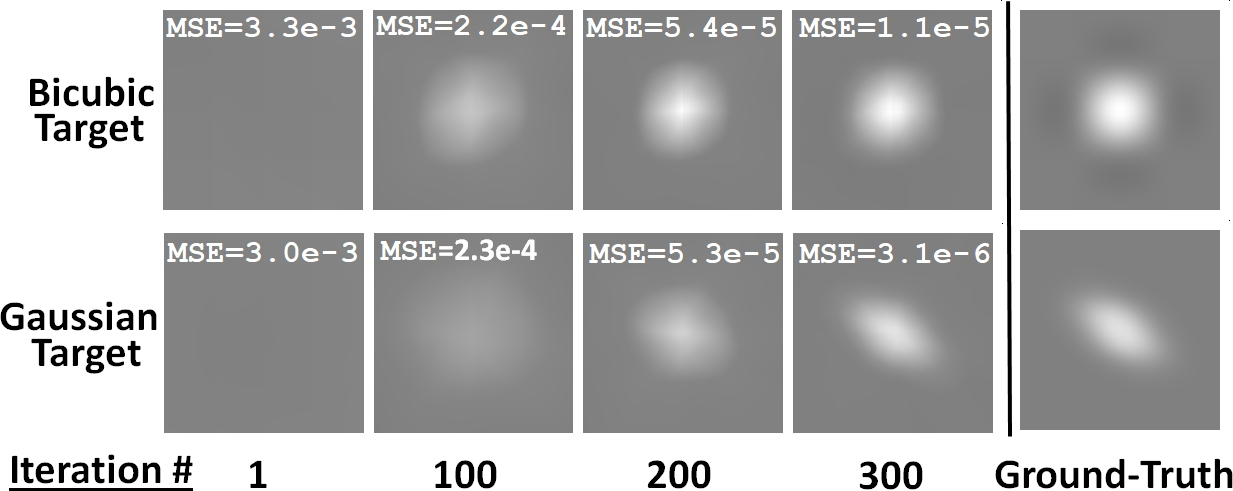
\includegraphics[width=1\textwidth]{figs/fig_visualize_Michal.jpg}
      \captionsetup{oneside, margin={-0.2cm,0cm}}
      \caption{\mbox{\it Visualizing the continuous learned kernels}}
      \label{fig:visualize}
    \end{minipage}
    \begin{minipage}{.4\textwidth}
        \vspace{-0cm}
        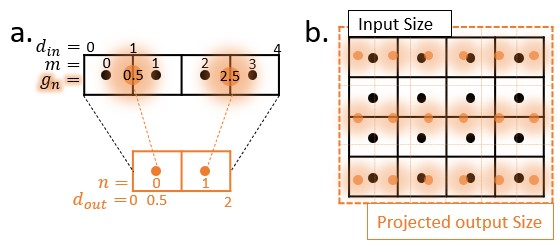
\includegraphics[width=1.5\textwidth]{figs/fig_grid.jpg}
        %\vspace*{0.5cm}
        \begin{minipage}{1.5\textwidth}
            \captionsetup{oneside, margin={1cm,0cm}}
            \caption{{\it The projected grid.}}
            \label{fig:grid}
         \end{minipage}%
    \end{minipage}%
    \vspace*{-0.5cm}
\end{figure}



\textbf{Block 2 -- Neighbors extraction:} For each grid point \varbold{$\textbf{g}_n$}, we now extract all its discrete nearest-neighbors $\varbold{\mathcal{N}[\textbf{n}]}$ \ben{from} $I$. These are all the input `pixels' centers within the support of the continuous kernel $\mathcal{K}_\theta$. This information is captured by a tensor of order 6 (blue tensor in Fig.~\ref{fig:overview}),  with shape $[N,1,C_{in},K,H',W']$ where K is the number of discrete neighbors in the kernel support. The second singleton dimension is for convenience in the next steps. We further need to extract the distances of each sub-`pixel' grid point \varbold{$\textbf{g}_n$} (of an output `pixel' {$\textbf{n}$}),  to all its discrete neighbors  ${\textbf{m}}\in I$. These distances $\varbold{\mathcal{D}[\textbf{n,m}]}$ are kept in a tensor $\varbold{\mathcal{D}}$ (shown in cyan in Fig.~\ref{fig:overview}), whose shape is $[K,2,H',W']$.

% Given a standard CNN input Tensor with dimensions Batch-size, Channels, Height and Width: $[N,C_{in},H,W]$.  We predefine support size (not necessarily an integer) for the continuous kernel $\mathcal{K}_\theata$. For each projected-grid point $\textbf{g'}$ we extract both values and distances to all input `pixels' within the kernel support. This stage produces a tensor consisting of all the neighbors values for each output `pixel'. This forces us to add a fifth dimension to the Neighbors tensor- the neighbors dimension. We actually extend this tensor to have 6 dimensions for convenience in the next stage, so the final shape is $[N,1,C_{in},K,H',W']$ where K is the number of neighbors in the kernel support. The Tensor of distances is shaped as a standard 2d CNN tensor, Its dimensions are: $[K,2,H',W']$. We use the batch dimension to distinguish between different neighbors. The second (channel) dimension is 2 to describe horizontal and vertical distances. Note that for simplicity, Fig.~\ref{fig:overview} depicts a case where $N=1, C_{in}=1$ and only the three last dimensions of the tensor are apparent.

% \textbf{Stage 3- Calculate weights:} The weights $\varbold{\mathcal{W}}$ are produced by the learnable model $\varbold{\mathcal{K}_\theta}$ applied to the distances tensor $\varbold{\mathcal{D}}$. 
\textbf{Block 3 -- Calculate weights:} The weights are produced by a learnable model $\varbold{\mathcal{K}_\theta}$, which is applied to the distances tensor:
%$\varbold{\mathcal{D}}$:
$\varbold{\mathcal{W} = \mathcal{K}_\theta \big\{ \mathcal{D}\big\}}$ (similarly to \cite{wang2018deep}).
A weight is assigned to connect between each output `pixel' and all its discrete input neighbors. Therefore, the weight tensor $\varbold{\mathcal{W}}$ will have a shape of $[1,C_{out},C_{in},K,H',W']$ 
(red tensor in Fig.~\ref{fig:overview}). 
%This tensor is marked in red in Fig.~\ref{fig:overview}. 
Its first singleton dimension is needed to match the size of the Neighbors tensor $\varbold{\mathcal{N}}$. As in standard conv, each output channel  $C_{out}$ is connected to all input channels $C_{in}$ through $\varbold{\mathcal{W}}$. We use a small neural network for $\varbold{\mathcal{K}_\theta}$ called the ``Internal-Net'' (marked in green in Fig.~\ref{fig:overview}). It is a simple CNN sequence of 1$\times$1 conv layers and ReLUs. This way every output `pixel' $\textbf{n}$ connects only to distances $\varbold{\mathcal{D}[\textbf{n}]}$ within its own set of discrete input neighbors. 

% The weights are produced by a learnable model which maps the distances calculated at stage 2 to corresponding weights for all the neighbors. This enforces consistency alongside expressivity. While each output `pixel' is calculated using a distinct local discrete kernel, all these local kernels are governed by the same underlying mapping function. We can choose to use a predefined fixed mapping, but we will usually use a learnable neural network, referred to as the internal-net. The input will be the distances tensor from preious stage. since we force the same mapping function to each output `pixel' we use several 1$\times$1 convolution layers and ReLUs in the internal-net. Consistency of the mapping to different neighbors is also enforced, since different neighbors are different instances in a batch. However, any model can be plugged to calculate the weights. Like in standard discrete convolutions, we have a set of continuous kernels, each maps all the input channels to an output channel. The weighted sum is actually taken not only over the neighbor values, but also over the input channels. Similarly to the neighbors tensor, the final weights tensor is of order 6: $[1,C_{out},C_{in},K,H',W']$ where the first dimension is the batch dimension which is always 1, to match the neighbors tensor.

\textbf{Block 4 -- Apply weights:} The final stage executes Eq.~\ref{eq:underlying} for the entire output tensor,
by multiplying the Weights tensor (red) with the Neighbors tensor (blue) and summing over all neighbors and input channels:
%. We simply multiply the Weights tensor (red) with the Neighbors tensor (blue) and sum over all the neighbors and input channels:
% For a given input feature-map $I$ of size $[N,C_{in},H,W]$, scale-factors $s_h, s_w$ and wanted shape $H',W'$ given at inference we finally get: 
\vspace*{-0.4cm}
\begin{align}
\varbold{I'}=
CC\{\varbold{I}\}= \sum_{c_{in}, k} \varbold{\mathcal{N}} \otimes \varbold{\mathcal{W}}
\end{align} 
with the following tensor shapes: 

$ \varbold{I'}:[N,C_{out},H',W'], \quad \varbold{\mathcal{N}}: [N,1,C_{in},K,H',W'], \quad \varbold{\mathcal{W}}:[1,C_{out},C_{in},K,H',W'] $

\subsection{Training and Generalization}
\label{sec:train}
CC is end-to-end trainable. The only trainable parameters of CC are $\varbold{\theta}$,  the parameters of $\varbold{\mathcal{K}_\theta}$. The gradient is propagated from the CC output through the weights tensor $\varbold{\mathcal{W}}$ to them. Gradients need to also be propagated to previous layers through the CC input. This is done easily through the neighbors extraction since it is just slicing (each neighbour neuron is actually a copy of an input neuron).

The output shape is determined by the shape of the grid $\varbold{{g}}$. Since $\varbold{\mathcal{K}_\theta}$ is a fully convolutional network, it can be applied to any spatial input size both at training and inference. This means that regardless of what sizes and scales we train on, a single CC, with a single set of parameters $\varbold{\theta}$ is applicable to any size and scale determined at real-time.

The input to  $\varbold{\mathcal{K}_\theta}$ is 
$\varbold{\mathcal{D}}$, which through the grid  $\varbold{{g}}$ depends only on the desired output scale \&
shape. Naturally, to generalize to many scales, we can sample various scales during training. However, being fully 1$\times$1 convolutional, $\varbold{\mathcal{K}_\theta}$ actually maps every 2D distance vector
%distance (two coordinates -- vertical and horizontal)
$\varbold{\mathcal{D}[\textbf{n,m}]}$ to a single value (weight) $\varbold{\mathcal{W}[\textbf{n,m}]}$. This means that $\varbold{\mathcal{D}}$ actually contains a huge batch of
inputs. This produces an interesting advantage: in almost all cases CC generalizes from one scale to any other scale. This happens as long as the diversity of distances in a single grid is reasonable. Eq.~\ref{eq:grid} suggests that if the scale is a rational number with a small numerator, 
then there exists only a small set of grid coordinates, and consequently a small set of unique distances $\varbold{\mathcal{D}[\textbf{n,m}]}$. For example, for $s=\nicefrac{1}{2}$ and a kernel with support of 2$\times$2, we get:
%\rightarrow 
$\varbold{\mathcal{D}[\textbf{n}]} = \Big\{(-\nicefrac{1}{2},-\nicefrac{1}{2}), 
(-\nicefrac{1}{2},\nicefrac{1}{2}), 
(\nicefrac{1}{2},-\nicefrac{1}{2}), 
(\nicefrac{1}{2},\nicefrac{1}{2})
\Big\} \ \ \varbold{\forall \textbf{n}}$, which will not generalize to other scales/distances. In other words, generalization occurs over the distribution of distances $\varbold{\mathcal{D}}$  between the grid points and `pixel' centers. If this distribution collapses to a small set of possibilities, then such generalization is damaged. However, training with a \emph{randomly} selected float scale-factor will give a huge diversity of sub-`pixel' distances in $\varbold{\mathcal{D}}$, hence will be able to generalize with very high probability to any other scale factor.
%\michal{Is this still true for large gaps between the train-scale  and the test-scale? After all, this will lead to a large difference in support size of K}. \assaf{supprt size of K is independent of the scale} 
Empirical evaluation of this property is described in the experiments section and in Fig.~\ref{fig:generalize}.
%\michal{Reference to Fig. 7 broken}
% \textbf{Cross-scale generalization:} Since the learning model $\mathcal{K}_\theta$ is unaware of the scale, it can be trained to one scale and generalize to another, under reasonable conditions. the scale trained on, cannot be a special case that collapses back to convolution, or a rational number with a denominator that is too small. In other words, generalization occurs over the distribution of distances between the grid and `pixel' centers. If this distribution collapses to a small set of possibilities then such generalization is damaged. A randomly selected float scale-factor will be able to generalize with probability ~1. 


% \textcolor{red}{
% \subsection{Training the CC-layer for dynamic scale generalization}
% \begin{itemize}[leftmargin=0.7cm]
% \item Please explain how to train the CC-layer so that it can generalize at test-time to any desired scale and shape.
% \item Please stress that although we use many scale/shape augmentations of the output layer, this is still a single trained network (as opposed to training multiple different networks, each for a different fixed output scale/shape). This is obvious to us, but may be a natural misconception of the reviewers, so it is worth stressing. Better safe than sorry...
% \end{itemize}
% }
\subsubsection{Experimental Settings}
\label{subsubsec:arxiv_cap_setting}




\paragraph{Dataset}
We divide ArXivCap into training and test sets with a 9:1 ratio for evaluation. The test set includes:
161.3K samples for single-figure captioning,
12.8K samples for multiple-figure captioning,
57.2K samples for contextualized captioning, and
57.2K samples for title generation.

\paragraph{Evaluated Models}
We select various LVLMs covering different architectures. 
(1) LVLMs designed for dealing with a single image, BLIP2-OPT-6.7B~\citep{li2023blip2}
, InstructBLIP-Vicuna7B~\citep{dai2023instructblip}, 
% MiniGPT4~\citep{zhu2023minigpt4}, 
LLaVA-1.5-7B/13B~\citep{liu2023llava15}. Due to the ability limitation, we only benchmark these models on the single image captioning task;
(2) LVLMs capable of handling interleaved text-image inputs, such as OpenFlamingo-9B~\citep{Alayrac2022FlamingoAV,awadalla2023openflamingo}, IDEFICS-Instruct-9B~\citep{laurencon2023obelics}, Qwen-VL-Chat-7B~\citep{Qwen-VL}. These models are evaluated on all the tasks we proposed;
(3) Proprietary models such as Gemini 1.0 Pro Vision and GPT-4V.
Due to the large scale of our test set, we randomly sample a subset consisting of 500 instances for evaluating these two models to reduce costs, with corresponding scores colored in \textcolor{gray}{grey}. Details of evaluated models and the task prompts used are provided in Appendix~\ref{apx:evaluation_details}.

\paragraph{Training Settings} 
To investigate whether in-domain training can enhance the model's capabilities, we train the Qwen-VL-Chat-7B on ArXivCap using the same setting as in \S\ref{subsubsec:exp_setting}. To fit the input length limit, we set the maximum number of figures per sample to four. The training process takes 70 hours with 8 NVIDIA A100s.
% To investigate whether in-domain training can enhance the model's ability, we train the Qwen-VL-Chat-7B for three epochs and adopt the AdamW optimizer~\citep{adam} with a learning rate of 1e-5 and weight decay set to 0.05, following the original setup of Qwen-VL-Chat.
% The dataset is split in a 9:1 ratio into training and test sets.
% We set the maximum figure number in a sample to $4$ to fit the input length limit.
% The training costs 70 hours with 8 NVIDIA A100 GPUs.

\paragraph{Metrics}BLEU-2~\citep{bleu}, ROUGE-L~\citep{lin-2004-rouge} and BERT-Score~\citep{bertscore} are adopted as the automatic evaluation metrics.
% We adopted BLEU-2 \citep{bleu}, ROUGE-L \citep{lin-2004-rouge}, and BERT-Score \citep{bertscore} as our automatic evaluation metrics. 
We also explore using GPT-4 to assist in caption evaluation. Our findings in Appendix \ref{apx:gpt4_eval} indicate that ROUGE-L and BLEU-2 scores are highly correlated with GPT-4's annotations. We primarily use these three metrics due to their convenience. A manual error analysis is conducted to supplement the automatic metrics~(\S\ref{subsubsec:manual_eval}).


% We also explore using GPT-4 to aid caption evaluation. Our results in Appendix~\ref{apx:gpt4_eval} show that ROUGE-L and BLEU-2 are highly correlated with the score annotated by GPT-4. We mainly use previous three metrics due to their convinence.
% Besides, a manual error analysis is performed to supplement the automatic evaluation (\S\ref{subsubsec:manual_eval}).
% As the automatic metrics cannot faithfully reflect the generation quality, we randomly sample pairs and perform human evaluation. We also incorporate GPT-4V for evaluation.


\begin{figure}[t!]
    \centering
    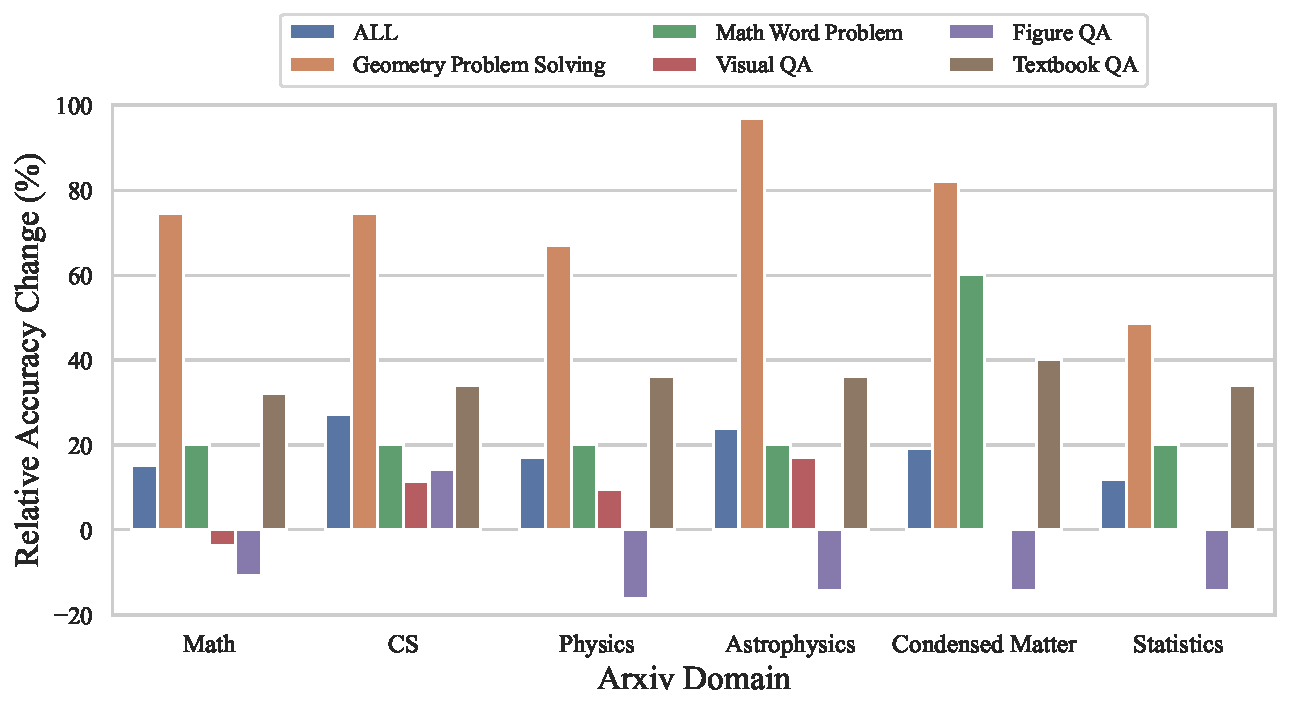
\includegraphics[width=\linewidth]{figs/domain_performance.pdf}
    \caption{Relative accuracy changes brought by the training on different domain ArXivQA samples.}
    \label{fig:domain_analysis}
\end{figure}
\begin{table}[t!]
    \centering
    \resizebox{\linewidth}{!}{
    \begin{tabular}{@{}l|ccc@{}}
    \toprule
    \textbf{Model}     &  BLEU-2 & ROUGE-L & BERT-S\\
    \midrule 
    % MiniGPT4 & & & \\ 
     BLIP-2-OPT-6.7B    & 2.1 & 7.1 & 81.1 \\ 
     InstructBLIP-Vicuna7B  & 3.7& 10.1 & 83.3 \\ 
     LLaVA-v1.5-7B    & 2.3 & 10.6 & 83.0 \\ 
     LLaVA-v1.5-13B    &2.6  & 10.7&  83.3 \\ 
      \midrule 
     OpenFlamingo-9B    & 5.7 &  9.9 & 82.4  \\ 
     IDEFICS-Instruct-9B & 2.5 & 9.1 & 83.5 \\ 
     Qwen-VL-Chat-7B &4.4 &11.1 & 81.8\\ 
     % + Title & & & \\ 
     % + Title and Abstract & & & \\ 
    Qwen-VL-Chat-7B$_\text{ArXivCap}$ & \textbf{8.9} & \textbf{15.8} & \textbf{83.3} \\ 
     % + Title & & & \\ 
     % + Title and Abstract & & & \\      
     \midrule
     % \textcolor{gray}{Bard} & \textcolor{gray}{3.4} & \textcolor{gray}{12.2} & \textcolor{gray}{82.2}\\ 
     \textcolor{gray}{Gemini 1.0 Pro Vision} & \textcolor{gray}{5.6} & \textcolor{gray}{14.5} & \textcolor{gray}{82.2}\\ 
     
        % \textcolor{gray}{GPT-4V} & \textcolor{gray}{5.7} &\textcolor{gray} {14.6}  & \textcolor{gray}{83.2}\\  200 subset 
      \textcolor{gray}{GPT-4V} & \textcolor{gray}{5.5} &\textcolor{gray} {14.2}  & \textcolor{gray}{83.3}\\  % 500 subset    
     \bottomrule
    \end{tabular}}
    \caption{Evaluation results of single figure captioning. \textcolor{gray}{Grey} results are obtained from a 500-sample subset. Despite most LVLMs struggle to produce high-quality captions of scientific figures, training with ArXivCap significantly boosts the performance.}
    \label{tab:single_cap_ret}
\end{table}
\begin{table}[t!]
    \centering
    \resizebox{\linewidth}{!}{
    \begin{tabular}{@{}l|ccc@{}}
    \toprule
    \textbf{Model}     &  BLEU-2 & ROUGE-L & BERT-S\\
    \midrule 
     Qwen-VL-Chat-7B &4.4 &11.1 & 81.8\\ 
      \quad + Title &5.7	&13.1&	81.6 \\ 
      \quad + Title and Abstract 	 & 6.0	 & 12.7	 & 81.4 \\ 
     \midrule 
    Qwen-VL-Chat-7B$_\text{ArXivCap}$ & 8.9 & 15.8 & 83.3 \\ 
     \quad + Title & \textbf{12.9}&	\textbf{18.6}	& \textbf{83.8} \\ 
      \quad + Title and Abstract &	12.7&	18.5&	83.8   \\      
     \bottomrule
    \end{tabular}}
    \caption{Evaluation results of single figure captioning with paper meta information.}
    \label{tab:cap_with_meta_ret}
\end{table}
\begin{table*}[tbh!]
\small 
\centering
\resizebox{\linewidth}{!}{
\begin{tabular}{@{}l|ccc|ccc|ccc@{}}
\toprule
\multirow{2}{*}{\textbf{Model}} & 
\multicolumn{3}{c}{\textbf{Multiple-Figure Captioning}}  & \multicolumn{3}{c}{\textbf{Contextualized Captioning}} & \multicolumn{3}{c}{\textbf{Title Generation}} \\
                       & BLEU-2 & ROUGE-L & BERT-S & BLEU-2 & ROUGE-L & BERT-S & BLEU-2 & ROUGE-L & BERT-S \\

% \midrule
% LLaVA-1          &      &       &            &      &       &            &      &       &            \\
% LLaVA-1.5       &      &       &            &      &       &            &      &       &            \\
% BLIP-2     &      &       &            &      &       &            &      &       &        \\
% InstructBLIP     &   0.0   &   10.1    &            &      &       &            &      &       &        \\
\midrule 
OpenFlamingo-9B  &     3.7  &  11.3     &  81.9           &    20.0  &     20.5  &         83.7  &    2.7   &   17.7    &  82.7      \\
IDEFICS-Instruct-9B &   3.6   & 10.8      &   82.8         & \textbf{20.7}   &     \textbf{22.6}  &     \textbf{85.7}        &    3.5    &     18.4 &     85.8    \\

Qwen-VL-Chat-7B   & 3.0     & 7.2   &  79.7          & 17.0   &   22.1  &  85.0         &  2.6    &     15.8  &   85.1         \\
 Qwen-VL-Chat-7B$_\text{ArXivCap}$ &  \textbf{10.6}     & \textbf{18.0}      & \textbf{83.6}           &    16.1    &    21.2     &        84.8     &     \textbf{6.7} &   \textbf{23.5}    & \textbf{86.8}      \\
\midrule
\textcolor{gray}{Gemini 1.0 Pro Vision}   &  \textcolor{gray}{6.1}    &   \textcolor{gray}{16.2}   &   \textcolor{gray}{83.1}     &  \textcolor{gray}{10.2}     &  \textcolor{gray}{20.2}       & \textcolor{gray}{84.5}           &   \textcolor{gray}{5.7}   &   \textcolor{gray}{21.8}  & \textcolor{gray}{85.9}     \\
\textcolor{gray}{GPT-4V}  &  \textcolor{gray}{5.7}   &  \textcolor{gray}{14.7}    &   \textcolor{gray}{83.0}         &    \textcolor{gray}{9.6}  &\textcolor{gray}{20.1}       & \textcolor{gray}{84.7}          &   \textcolor{gray}{4.0}   &   \textcolor{gray}{20.2}  &   \textcolor{gray}{86.0}     \\
% \textcolor{gray}{Bard}  &      &       &            &      &       &            &      &       &        \\
\bottomrule
\end{tabular}
}
\caption{Evaluation results of three newly defined tasks. The best results are highlighted in \textbf{bold}.}
\label{tab:ret_three_tasks}
\end{table*}
\subsubsection{Results}
\paragraph{Results of Single-Figure Captioning}
The evaluation results for the single-figure captioning task are presented in Table \ref{tab:single_cap_ret}. Despite achieving near-perfect performance on conventional image captioning tasks like MSCOCO \citep{lin2014mscoco}, open-source LVLMs, such as LLaVA models, face challenges when applied to academic figures. 
% Among the LVLMs, Qwen-VL-Chat emerges as the top-performing open-source candidate, surpassing its counterparts. 
For closed models, GPT-4V performs comparably with Gemini 1.0 Pro Vision.
Furthermore, continuous training on our dataset yields a significant performance boost for this task. For instance, fine-tuning results in a notable increase in the BLEU-2 score from 4.4 to 8.9, indicating a promising avenue for enhancing academic figure comprehension through domain-specific training.
We also investigate whether providing additional context information, such as the paper title and abstract, could help models generate better figure captions. As shown in Table \ref{tab:cap_with_meta_ret}, adding the title is beneficial evidenced by the boosted scores, while providing abstracts brings negligible gains.

% The evaluation results for the single figure captioning task are presented in Table~\ref{tab:single_cap_ret}. 
% Despite achieving almost perfect performance on conventional image captioning tasks such as MSCOCO~\citep{lin2014mscoco}, LVLMs encounter challenges when applied to academic figures. Among LVLMs, Qwen-VL-Chat emerges as the top-performing open-source candidate, surpassing its counterparts. 
% GPT-4V performs comparably with the Gemini 1.0 Pro. 
% Moreover, continuous training on our dataset yields a significant performance boost for this task. For instance, fine-tuning results in a notable increase in the BLEU-2 score from 4.4 to 8.9, indicating a promising avenue for enhancing academic figure comprehension through domain-specific training.
% We further investigate whether providing additional context information such as paper title and abstract could help models caption figures better.
% As shown in Table~\ref{tab:cap_with_meta_ret}, adding the title is beneficial for generating better captions while providing abstracts seems to bring negligible gains.

\paragraph{Results of Multiple-Figure Captioning}
As shown in the first block of Table \ref{tab:ret_three_tasks}, similar to single-figure captioning, multiple-image captioning poses a challenge for current open-source LVLMs. For instance, Qwen-VL-Chat achieves only a 3.0 BLEU-2 and a 7.2 ROUGE-L score on this task, considerably lower than its performance in single-figure captioning. In contrast, GPT-4V consistently demonstrates proficiency in both tasks, suggesting a balanced ability to capture semantics across multiple images. Notably, training on our ArXivCap dataset yields more pronounced improvements for this task, culminating in Qwen-VL-Chat even surpassing the performance of the GPT-4V model. This enhancement underscores the pivotal role of our dataset in facilitating LVLMs to enhance reasoning capabilities over multiple images, leading to more effective summarization of scientific figures.

\paragraph{Results of Contextualized Captioning}
In the middle block of Table~\ref{tab:ret_three_tasks}, we find that IDEFICS-Instruct-9B achieves the best performance on this task.
This achievement is largely attributed to its remarkable proficiency in leveraging contextual cues, stemming from its extensive pre-training involving interleaved image-text pairs~\citep{laurencon2023obelics}. 
Interestingly, fine-tuning on ArXivCap results in marginal performance declines across all metrics, with GPT-4V achieving the lowest scores as well. 
This phenomenon can be attributed to the tendency of sequential captions to exhibit similar patterns, thereby favoring models that effectively leverage contextual cues.
% such as copying previous captions.
% Interestingly, fine-tuning on ArXivCap leads to marginal performance declines across all metrics and GPT-4V achieves the lowest scores as well.
% We attribute this phenomenon to the fact that sequential captions usually have similar patterns, therefore models that pay more attention to contextual cues can obtain higher scores.
% We hypothesize that the fine-tuned model would focus more on the image content instead of referring to the previous captions when generating the new caption. 
We perform two more challenging evaluations by (i) providing context pairs from another paper and (ii) randomly shuffling the order of figure-caption pairs in the context.
As shown in Table~\ref{tab:order_analysis}, 
the performance with random contexts degrades significantly, validating our previous hypothesis.
Instead, the fine-tuned model demonstrates more robust captioning results under these settings, evidenced by the slight 8\% drop on ROUGE-L compared to the 31\% of the original model with shuffled context orders.


\begin{table}[t!]
    \centering
    \resizebox{\linewidth}{!}{
    \begin{tabular}{l|cc}
    \toprule
       Model  &   BLEU-2 ($\Delta\downarrow$) & ROUGE-L ($\Delta\downarrow$)  \\
    \midrule
        Qwen-VL-Chat-7B & 17.0 & 22.1\\ 
       \quad + random contexts & 	5.7 (66.5\%)&  13.0 (38.1\%)\\ 
       \quad  + shuffle order& 12.0 (29.4\%) &15.1 (31.7\%) \\ 
       
    \midrule 
      Qwen-VL-Chat-7B$_\text{ArXivCap}$ & 16.1 & 21.2\\ 
       \quad + random contexts	& 7.5 (53.4\%)	& 14.3 (32.5\%)\\ 
        \quad + shuffle order & 14.1 (12.4\%) & 19.5 (8.0\%) \\
    
    \bottomrule
    \end{tabular}}
    \caption{Contextualized captioning performance is influenced by the order. After tuning on the ArXivCap, the model is more robust to the order of the history captions.}
    \label{tab:order_analysis}
\end{table}
\paragraph{Results of Title Generation}
The results are presented in the last block of Table~\ref{tab:ret_three_tasks}.
Notably, the title generation task poses a formidable challenge, evident in the significantly lower overall BLEU-2 score compared to the captioning tasks. This suggests the inherent difficulty in generating precise predictions for paper titles.
% We observe that for the title generation task, the overall BLEU-2 score is much lower than the captioning tasks, indicating that it is challenging to generate the exact prediction for the paper. 
A contrasting picture emerges when considering the ROUGE-L and BERT-Score metrics, which either closely align or surpass the performance on captioning tasks. This underscores the model's proficiency in producing semantic-related results given the presented figures. 
Consistent with the previous two tasks,
fine-tuning the model on our dataset yields substantial enhancements for the title generation task. The BLEU-2 score jumps impressively from 2.6 to 6.7, while the ROUGE-L score sees a commendable increase from 15.8 to 23.5. 
These findings highlight the challenge of title generation for current LVLMs and the effectiveness of our dataset in improving the model's capability to generate accurate titles.

% Consistent with the previous two tasks, fine-tuning the model on our dataset also brings a clear improvement for the title generation, increasing the BLEU-2 score from 2.6 to 6.7 and ROUGE-L score from 15.8 to 23.5.


% \subsection{Analysis}
% In this section, we further perform additional analysis to understand the bottleneck of existing models.


% \paragraph{Pure Text2Text Model}
% OCR analysis 
% add results on the OCR t

% \paragraph{Prompt Sensitivity}
% \paragraph{Order Sensitivity of Contextualized Captioning}


% \paragraph{Transfer to Science QA dataset}

\subsection{Analysis}

\begin{figure}
    \centering
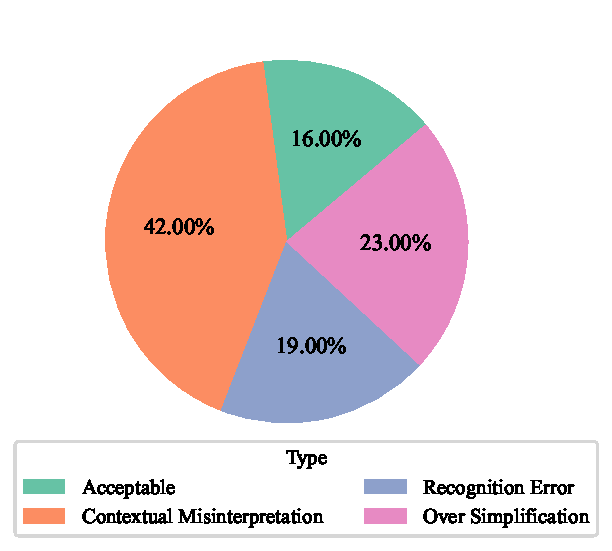
\includegraphics[width=0.8\linewidth]{figs/pie_chart.pdf}
    \caption{Manual analysis of the generated captions. }
    \label{fig:error_pie_chart}
\end{figure}


\begin{figure*}
    \centering
    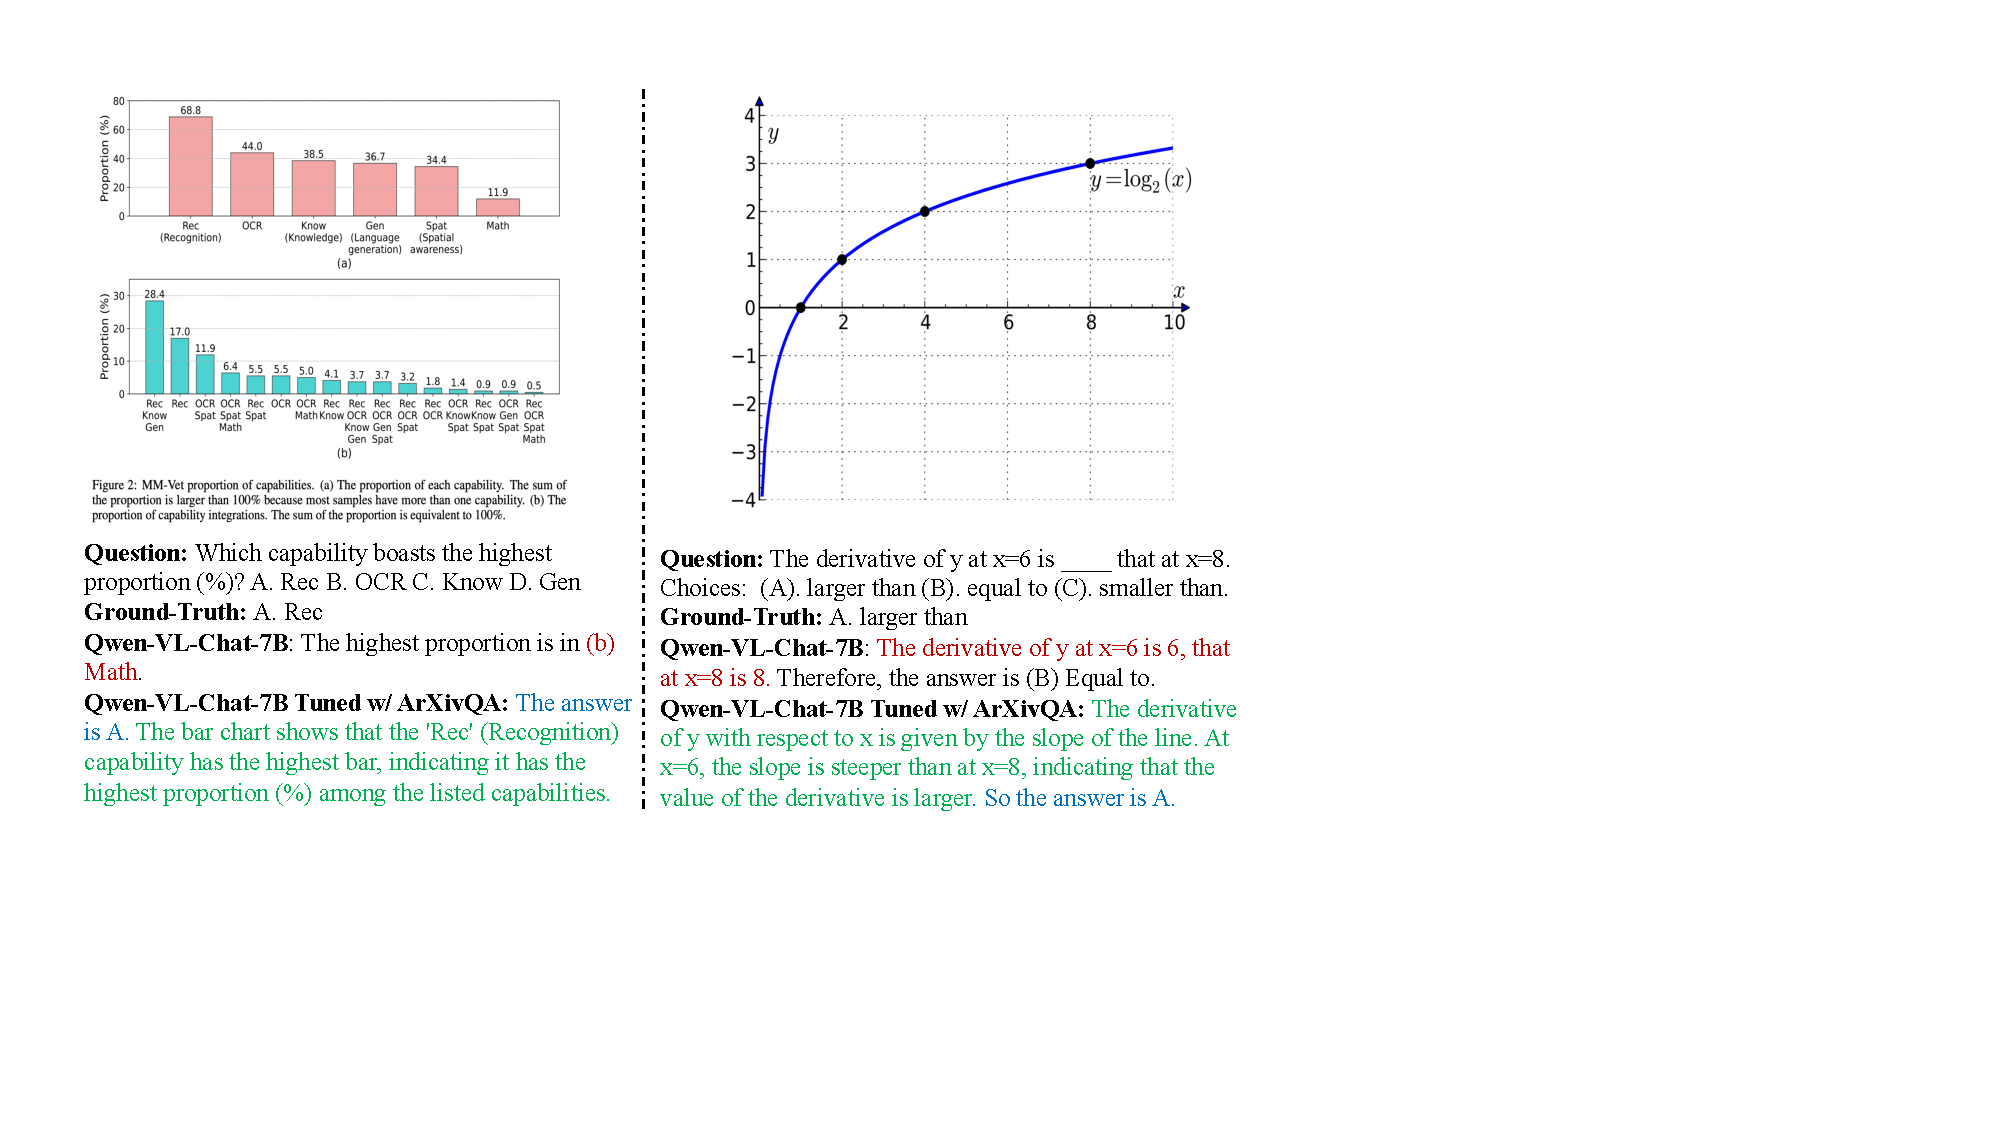
\includegraphics[width=0.62\linewidth]{figs/mathvista_case_study_v2.pdf}
    \caption{ArXivQA enables the model not only to answer questions related to scientific figures in papers (left) but also to improve mathematical understanding ability (right). The model not only selects correct options but also gives reasonable rationale.}
    \label{fig:math_case_study}
\end{figure*}

\paragraph{Manual Evaluation of Generated Captions} 
\label{subsubsec:manual_eval}
We conduct a manual inspection for single-figure captioning results. To ensure a more informed evaluation, we focus on a paper from the CS domain, leveraging our domain knowledge to assess caption quality better. 
The quality of generated captions is assessed by scrutinizing the figure, the ground-truth caption, the paper title, and the abstract.
We categorize captions into the following quality types according to our preliminary inspection: (1) \emph{Acceptable}, where captions accurately encapsulate the scientific figure's essence, aligning with the intended information of the ground-truth; (2) \emph{Over Simplification}, instances where the model oversimplifies content, offering a broad overview while neglecting specific details and nuances present in the ground truth; (3) \emph{Recognition Error}, where the model inaccurately recognizes and describes key visual and textual elements in the scientific figure, such as colors, numerical values, or textual context; and (4) \emph{Contextual Misinterpretation}, where the model misinterprets the specific context of the scientific figure, resulting in captions relevant in a generic sense but inaccurate for the given figure. Visualized generated captions of different types are shown in Figure~\ref{fig:caption_type} of Appendix~\ref{apx:caption_type}.
The results of 100 manually examined captions are depicted in Figure~\ref{fig:error_pie_chart}, revealing that only 16\% of captions are deemed acceptable when compared to human-written ones. 
Among unsatisfactory captions, contextual misinterpretation emerges as the dominant issue, suggesting a need for incorporating more contextual information as suggested in Table~\ref{tab:cap_with_meta_ret}. Oversimplification is another concern, with generic captions identified. Additionally, 23\% and 19\% of examined captions suffer from the oversimplification issue and recognition errors in reported numbers/texts in the caption, respectively. The former is attributed to the highly frequent simple caption in the training dataset and the latter issue could be addressed through potential integration with OCR results.
% In summary,  underscores opportunities to enhance captioning quality. 
Our manual evaluation suggests future efforts may benefit from incorporating additional context clues, such as paper metadata, improving the model's fundamental perception abilities, and utilizing external information.


% The error distribution comes from Figure~\ref{fig:error_pie_chart} shows that 16\% of the captions are perceived as acceptable compared with the human-written ones, indicating sufficient room for further improvements.
% Among the unsatisfactory captions, the most dominant type is contextual misinterpretation, which could be alleviated by incorporating more contextual information.
% Another issue is oversimplification, where the captions are generic to the present figure, such as (a) in Figure X.
% Also, 19\% of examined captions suffer from the recognition ability of the base model, i.e., the numbers are wrongly reported, which we think can be combined with OCR results.
% In summary, our manual evaluation suggests that future endeavors can be conducted to improve the captioning quality by incorporating more context clues, such as meta data of the paper, and improve the fundamental perception ability of the model.
% Acceptable 0.16
% Over Simplification 0.23
% Contextual Misinterpretation 0.42
% Recognition Error 0.19


\paragraph{Case Study of MathVista}
We conduct case studies to illuminate the tuning effects facilitated by our ArXivQA dataset. In the left segment of Figure~\ref{fig:math_case_study}, ArXivQA helps the model accurately answer a question related to the presented bar plot. 
% Notably, our ArXivQA, rooted in figures extracted from scientific papers, extends its impact beyond visual data. 
The right part in Figure~\ref{fig:math_case_study} demonstrates that ArXivQA can enhance algebraic reasoning abilities. Here, a question involving the derivative of a function is correctly answered, accompanied by a lucid reasoning rationale.
Figure~\ref{fig:geometry_fail} in Appendix~\ref{apx:failure_mathvista} highlights a challenging geometry problem where both models generate hallucinated outputs. 
These illustrative cases collectively affirm the efficacy of our dataset.
% reinforcing the observed quantitative accuracy improvements. 
% These nuanced examinations not only provide a qualitative understanding of the tuning effects but also underscore the dataset's broader impact on diverse mathematical reasoning tasks.


% We further present case studies to understand the improvement of the tuning effect of our ArXivQA dataset. As shown in the left part of Figure~\ref{fig:math_case_study}, the model after fine-tuning produces a correct answer for the question related to the presented bar plot. While our ArXivQA is constructed based on the figures extracted from scientific papers, the right case in Figure~\ref{fig:math_case_study} suggests that fine-tuning may also improve the algebraic reasoning ability, where a question of function derivative is correctly answered with reasoning rationale.
% We also present a failed geometry problem in Figure~\ref{fig:geometry_fail} in the Appendix where we found both models produce hallucinated outputs for a challenging geometry problem. Overall, these intuitive cases confirm the effectiveness of our dataset, echoing previous quantitative accuracy boost.